\chapter{Simulation}
\thispagestyle{empty}
\label{chap6}

Circuit simulation \index{Circuit simulation} uses mathematical models
to replicate the behaviour of an actual device or circuit. Simulation
software allows to model circuit operations. Simulating a
circuit's behaviour before actually building it can greatly improve
design efficiency. eSim uses {\tt Ngspice}\index{Ngspice} for analog, digital and
mixed-level/mixed-signal circuit simulation. The various steps involved in simulating a circuit schematic in eSim are explained in the sections below:

\section {Kicad to Ngspice Conversion}
In the chapter on schematic creation, we have learnt to generate the netlist from circuit schematic. The generated netlist is not compatible with Ngspice. eSim uses Ngspice to simulate the circuit schematic. Hence the netlist i.e. {\tt .cir} file generated should be converted in to a  Ngspice compatible file. The \textit{Convert KiCad to Ngspice} tool on eSim left toolbar is used to do this. Let us now see the various tabs and their functions available under this.   

\subsection {Analysis} \label{ana}
In order to simulate a circuit, the user must define the type of
analysis to be done on the circuit. This tab is used to insert the type of analysis and  value of the analysis parameters to the netlist. eSim supports three types of analyses:
\begin{inparaenum}
\item \textit {DC Analysis} (Operating Point and DC Sweep) \index{DC Analysis}
\item \textit {AC Small-signal Analysis} \index{AC Small-signal Analysis} 
\item \textit {Transient Analysis} \index{Transient Analysis}
\end{inparaenum}
These are explained below. %\cite{ngspice}.

\begin{figure}
\centering
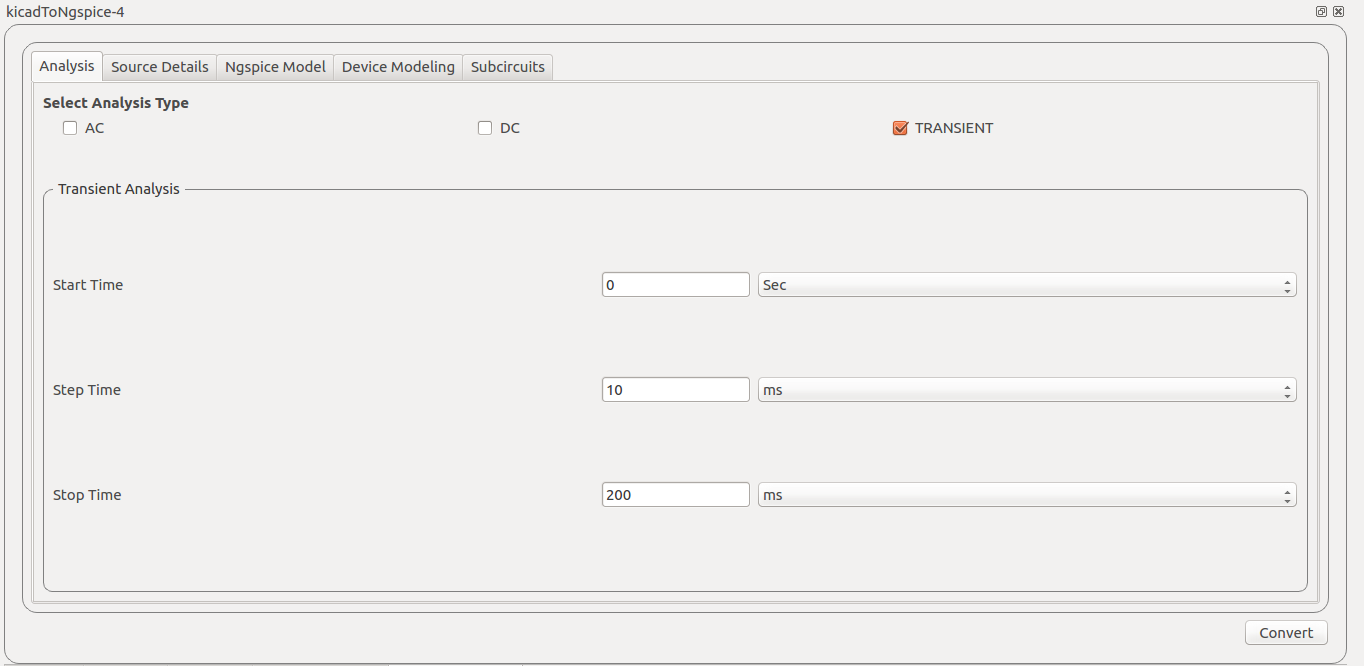
\includegraphics[width=\lgfig]{analysis.png}
\caption{KiCad to Ngspice Window}
\label{analysis}
\end{figure}

In the current example for simulating an RC circuit, select the analysis type as {\tt transient} analysis and enter the values as shown in the \figref{analysis}.  

\begin{comment}
Analysis Inserter generates the commands for Ngspice. When one clicks
on \textit {Kicad to Ngspice} from the eSim toolbar, one gets
the Analysis Inserter GUI as shown in \figref{1}. The various tabs in
this GUI correspond to the various types of analysis. The user can
enter the details, needed to perform simulation, in the corresponding
fields under these tabs.

\subsubsection{DC analysis} \index{DC Analysis} The {\tt DC analysis}
determines the dc operating point of the circuit with inductors
shorted and capacitors opened. It is assumed that there is no time dependence on any of the sources within the system description. The simulator algorithm subdivides the circuit into those portions which require the {\tt analog simulator algorithm} and
those which require the {\tt event-driven algorithm}. Each subsystem block
is then iterated to solution, with the interfaces between analog nodes
and event-driven nodes iterated for consistency across the entire
system. Once stable values are obtained for all nodes in the system, the
analysis halts and the results could be displayed or printed out.
 
A {\tt DC analysis} is automatically performed prior to a {\tt transient analysis}
to determine the transient initial conditions, and prior to an {\tt ac
small-signal analysis} to determine the linearized, small-signal models
for nonlinear devices.  The {\tt DC analysis} can also be used to generate
dc transfer curves: a specified independent voltage or current source
is stepped over a user-specified range and the dc output variables are
stored for each sequential source value.

\subsubsection{AC small-signal analysis}\index{AC Small-signal Analysis}
{\tt AC analysis} is limited to analog nodes. It represents the small
signal, sinusoidal solution of the analog system described at a
particular frequency or set of frequencies. This analysis is similar
to the {\tt DC analysis} in that it represents the steady-state behaviour of
the described system with a single input node at a given set of
stimulus frequencies.

The program first computes the dc operating point of the circuit and
determines linearized, small-signal models for all of the nonlinear
devices in the circuit. The resultant linear circuit is then analyzed
over a user-specified range of frequencies. The desired output of an
ac small-signal analysis is usually a transfer function (voltage gain,
trans impedance, etc.). If the circuit has only one ac input, it is
convenient to set that input to unity and zero phase, so that output
variables have the same value as the transfer function.

\subsubsection{Transient analysis}\index{Transient Analysis}
{\tt Transient analysis} is an extension of {\tt DC analysis} to the time
domain. A {\tt transient analysis} begins by obtaining a DC solution to
provide a point of departure for simulating time-varying
behaviour. Once the DC solution is obtained, the time-dependent aspects
of the system are reintroduced and the simulator algorithms
incrementally solve for the time varying behaviour of the entire
system. Inconsistencies in node values are resolved by the simulation
algorithms such that the time-dependent waveforms created by the
analysis are consistent across the entire simulated time interval.

Resulting time-varying descriptions of node behaviour for the specified
time interval are accessible. All sources which are not time
dependent (for example, power supplies) are set to their dc value. The
transient time interval is specified on a \textit {.tran} control line.  


\subsection{DC analysis inserter}
By default {\tt DC analysis} option appears when one clicks on \textit {Analysis
Inserter}. Here we need to give the details of input \textit {source name}, \textit {start
value} of input, \textit {increment} and \textit {stop} value. Once this is done, click on \textit {Add
Simulation Data}.

\figref{2} gives an example of {\tt DC analysis} inserter.  In this example,
{\tt v1} is the input voltage source which \textit {starts} at {\tt 0
  Volt}, \textit {increments} by {\tt 1 Volt} and \textit {stops} at
{\tt 10 Volt}. On clicking \textit {Add Simulation Data}, the analysis
command is generated and is of the form:
\\
{\tt.dc\index{.dc} sourcename vstart vstop vincr}
\\
The {\tt .dc} line defines the dc transfer curve source and sweep
limits (with capacitors open and inductors shorted). {\tt srcnam} is
the name of an independent voltage or current source. {\tt vstart},
{\tt vstop}, and {\tt vincr} are the starting, final, and incrementing
values respectively, of the source.

When we check the option \textit {Operating Point
  analysis}\index{Operating point analysis} on the DC analysis window,
{\tt .op} gets appended to the analysis statement.
\begin{figure}[ho]
\centering
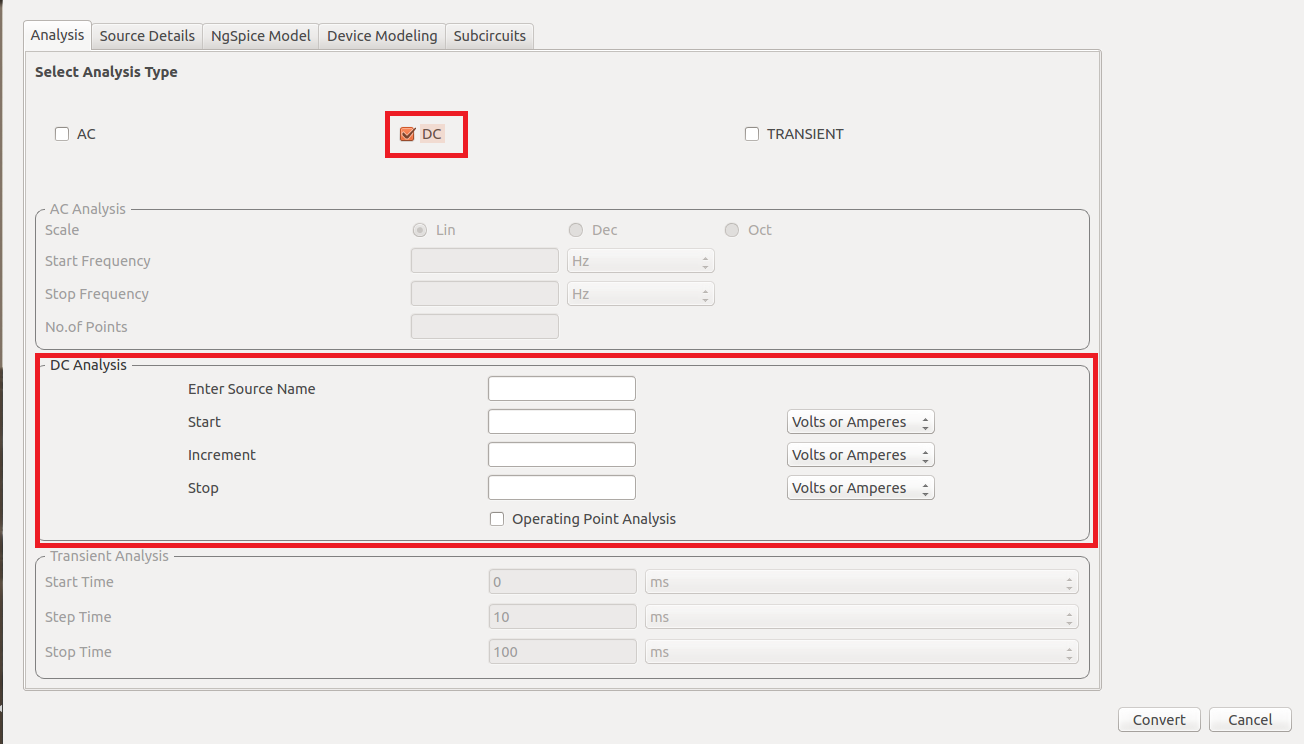
\includegraphics[width=0.475\linewidth]{figures/dc1.png}
\caption{DC Analysis GUI}
\label{2}
\end{figure}
The inclusion of the line {\tt .op} in the analysis file directs
Ngspice to determine the dc operating point of the circuit with
inductors shorted and capacitors opened.

\subsection{AC analysis inserter}\index{AC Analysis Inserter}
When one clicks on the option \textit {AC} in the \textit {Analysis Inserter} GUI, the
window given in \figref{4} appears.
\begin{figure}[ho]
\centering
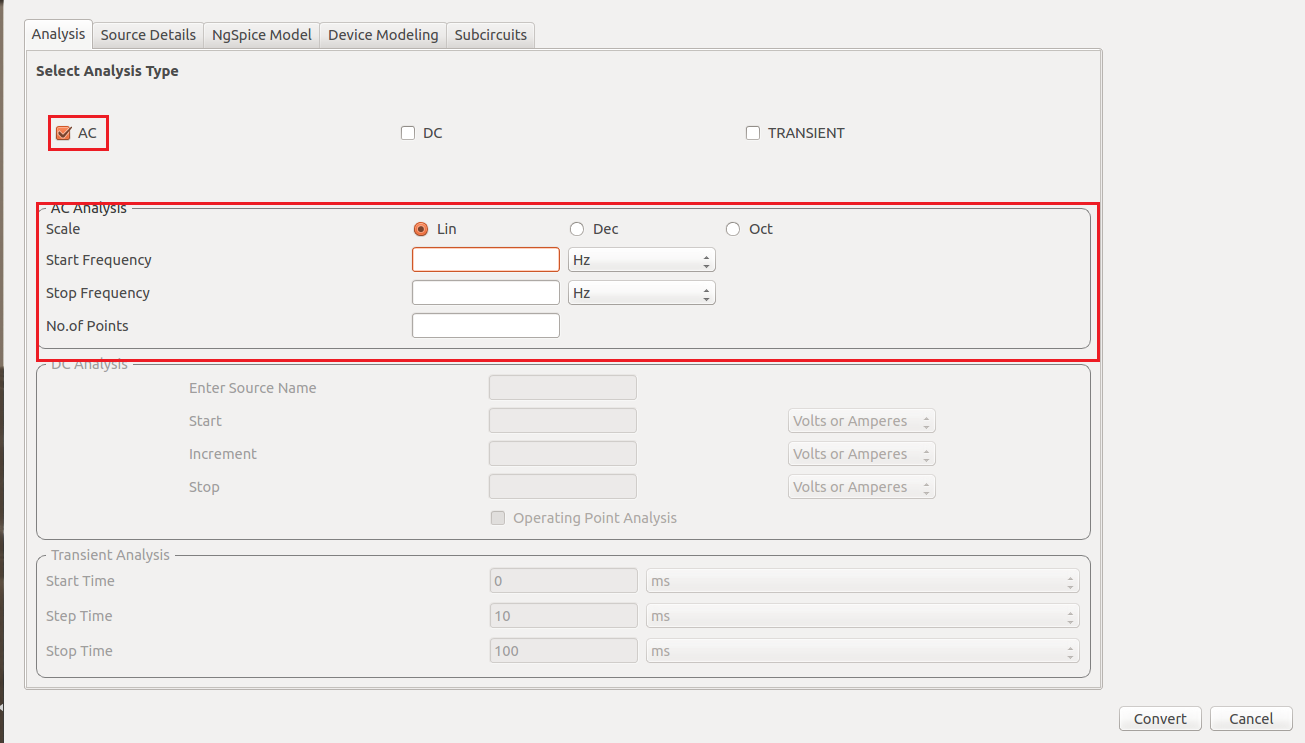
\includegraphics[width=\smfig]{figures/ac1.png}
\caption{AC Analysis GUI}
\label{4}
\end{figure}
Here one needs to enter the details of \textit {scale}, \textit {start
  frequency}, \textit{stop frequency} and \textit {Number of points}. 

After entering these values, click on \textit {Add Simulation
  Data}. The analysis statement is generated. This is in one
of the three forms listed below, depending on the type of \textit
{scale} that one chooses. The types of \textit {scale} available are
\textit {dec}, \textit {oct}, and \textit {lin}, the usage of which is
explained below: \\
{\tt .ac dec nd fstart fstop }\\
{\tt .ac oct no fstart fstop }\\
{\tt .ac lin np fstart fstop } \index{.ac} \\
Here, {\tt dec} stands for decade
variation and {\tt nd} is the number of points per decade. {\tt oct}
stands for octave variation and {\tt no} is the number of points per
octave. {\tt lin} stands for linear variation and {\tt np} is the number of
points. {\tt fstart} is the starting frequency and {\tt fstop} is the
final frequency.

If the {\tt .ac} analysis is included in the analysis file, Ngspice
performs an AC analysis of the circuit over the specified frequency
range. Note that in order for this analysis to be meaningful, at least
one independent source must have been specified with an ac value. While creating the schematic for performing ac analysis, add the component {\tt AC} from the \textit{sourcesSpice} library.

\subsection{Transient analysis inserter}\index{Transient Analysis
  Inserter}
When one clicks on the option \textit {Transient} in the \textit {Analysis Inserter}
GUI, the window given in \figref{6} appears.  Here one needs to
enter the details of \textit {start time}, \textit {step time}, and \textit {stop
  time}.  After entering these values, click on \textit {Add Simulation
Data}. The analysis statement is generated. It is of the
form:

{\tt .tran tstep tstop tstart}\index{.tran}

Here, {\tt tstep} is the printing or plotting increment for
line-printer output. For use with the post-processor, {\tt tstep} is
the suggested computing increment. {\tt tstop} is the final time, and
{\tt tstart} is the initial time. If tstart is omitted, it is assumed
to be zero.

The transient analysis always begins at time zero. In the interval
{\tt \textless zero, tstart\textgreater}, the circuit is analyzed (to
reach a steady state), but no outputs are stored. In the interval {\tt
  \textless tstart, tstop\textgreater}, the circuit is analyzed and
outputs are stored.
\begin{figure}[ho]
\centering
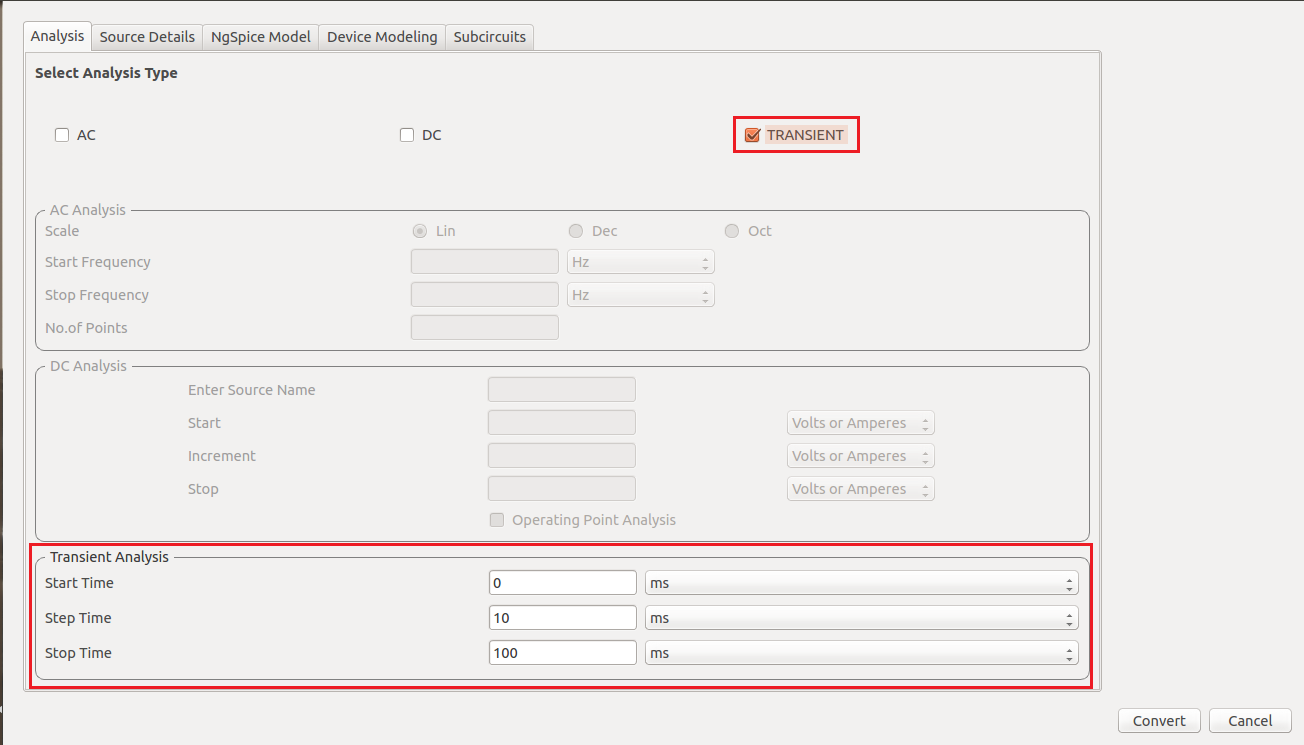
\includegraphics[width=\smfig]{figures/trans1.png}
\caption{Transient Analysis GUI}
\label{6}
\end{figure}


\begin{enumerate}
\item \textit {Analysis} - This tab is used to insert the type of analysis and  value of the analysis parameters to the netlist.
\item \textit {Source Details} - The netlist created in the \textit{Schematic Editor} is converted to 
  Ngspice format and analysis commands is appended to it. It is done
  by the \textit{Netlist Converter} tool in the eSim
  toolbar. \index{Netlist Converter}
\item Ngspice Modelling \index{Ngspice simulation} - Ngspice
  simulation of the netlist is performed. It is done by clicking on the \textit{Ngspice} tool in the eSim toolbar.
\item Model Library - Model library adds the component library of the components like Diode, JFET, MOS, IGBT. These library file contains the parameters and the values of the components.

\item Sub-Circuit - A sub circuiting can be done using this tool. This involves adding the sub circuit used in the main circuit. This adds all the project files of the sub circuit.
\end{enumerate}
\end{comment}

\subsection {Source Details} \label{source}
The various parameter values of the sources added in the schematic can added using this tool. \textit {Source details} is a dynamic tab, i.e. the fields are added as per the number of sources in the circuit. For example, consider a Half-Adder circuit as shown in \figref{halfschematic}
\begin{figure}
\centering
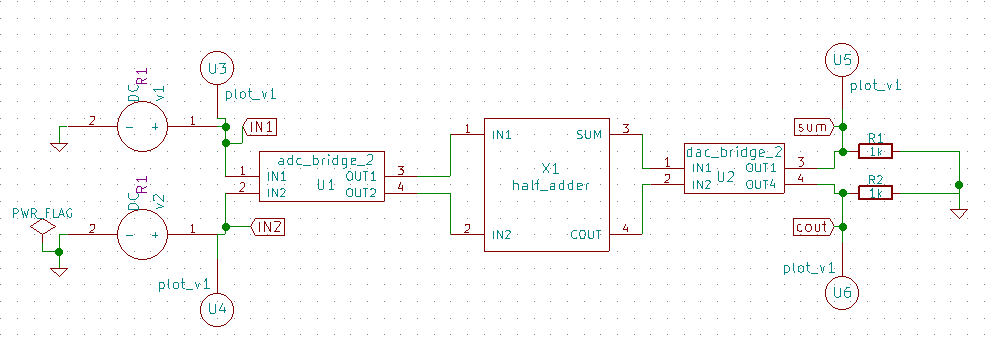
\includegraphics[width=\lgfig]{manual_images/half-adder.png}
\caption{Half Adder Schematic}
\label{halfschematic}
\end{figure}
Here, we have used two DC input sources are used and hence the source detail GUI would be having two input fields as shown is \figref{sourcehalfadder}.

\begin{figure}[h]
\centering
\subfloat[Source Details of Half-Adder]{
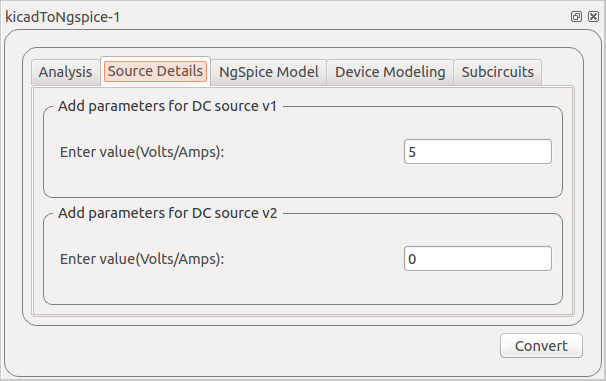
\includegraphics[width=\smfig]{manual_images/source-details.png}
\label{sourcehalfadder}} \hfill
\subfloat[Source Details of RC circuit]{
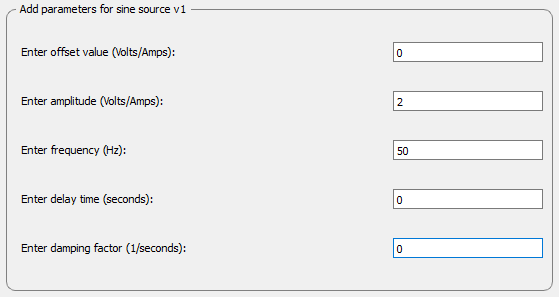
\includegraphics[width=\smfig]{manual_images/rc-sourcedetails.PNG}
\label{sourcerc}} \hfill
\caption{Source details interface}
\end{figure}

In the current example of the RC circuit, we have a single AC source. Fill in the details as shown in \figref{sourcerc}.

\subsection {Ngspice Model} \label{ngspicemodel}
The component libraries for components like DAC, ADC, transformer etc. which are used in the schematic are directly linked with the corresponding Ngspice models. The user can modify the parameter values using this tab, as shown in \figref{ngspicemodel}. If there are no modifications the default values are taken.

\begin{figure}
\centering
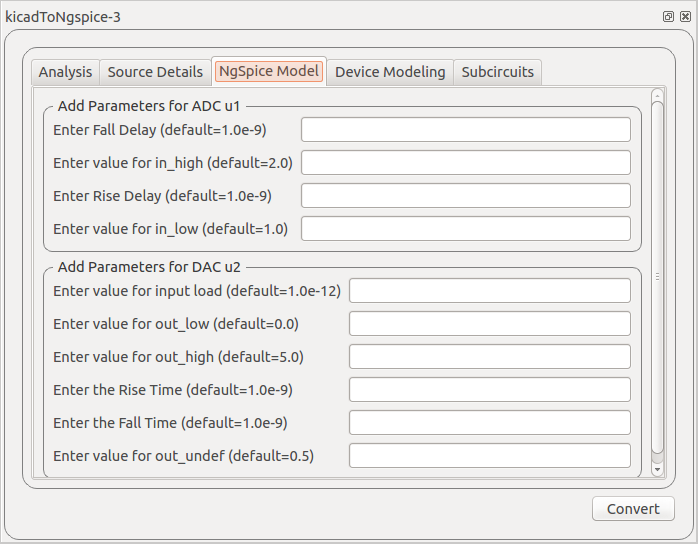
\includegraphics[width=\lgfig]{manual_images/ngspice-model.png}
\caption{Half adder: Ngspice model}
\label{ngspicemodel}
\end{figure}

\subsection {Device Modelling} \label{devicemodel}
Spice based simulators include a feature which allows accurate modeling of semiconductor devices such as diodes, transistors etc. Model libraries holds these features to define models for devices such as diodes, MOSFET, BJT, JFET, IGBT, Magnetic core etc.

The fields in this tab are added for each such device in the circuit and the corresponding model library is added. In the example of bridge rectifier as shown in \figref{bridgerectifier} for four diodes library files are added as in \figref{devicemodel}. Location for these libraries is as following : \\
library/deviceModelLibrary/Diode/ if you are using version 2.0 and above \\
src/deviceModelLibrary/Diode/ if you are using versions lower than 2.0

\begin{figure}[h]
\centering
\subfloat[Schematic]{
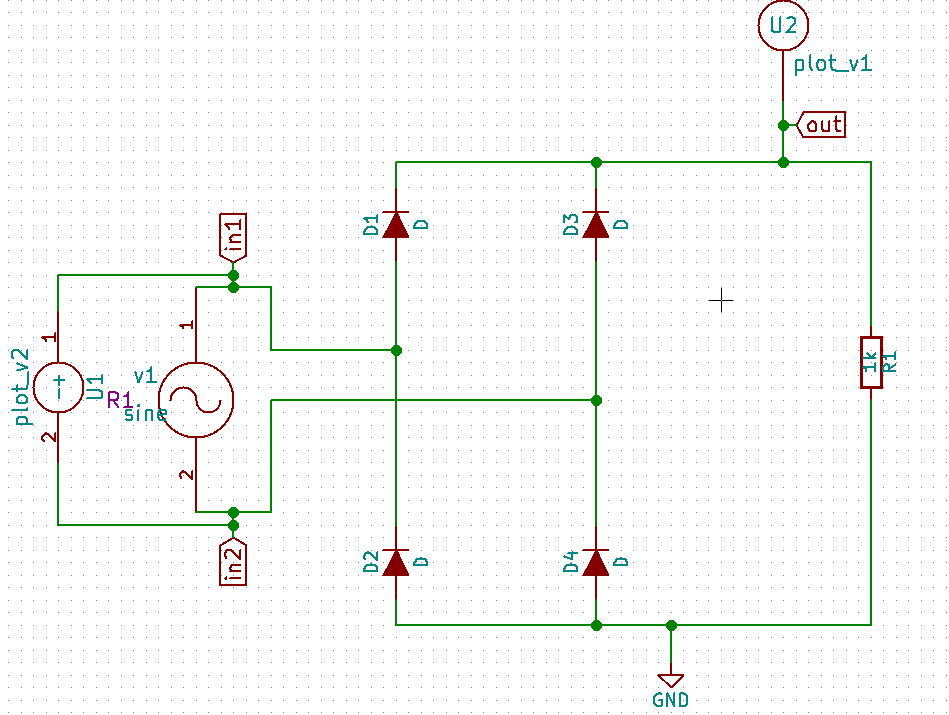
\includegraphics[width=\smfig]{manual_images/bridgerectifier.png}
\label{bridgerectifier}} \hfill
\subfloat[Adding device model]{
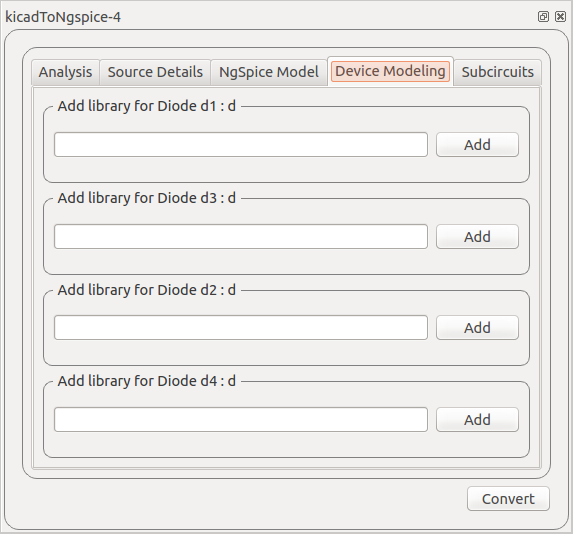
\includegraphics[width=\smfig]{manual_images/devicemodel.png}
\label{devicemodel}} \hfill
\caption{Bridge Rectifier}
\end{figure}

\subsection{Sub Circuit}
Subcircuit is a way to implement hierarchical modeling.  Once a subcircuit for a compo-
nent is created, it can be used in other circuits. \\
In the KiCadToNgspice conversion of example 7805VoltageRegulator, where a bridge rectifier is further connected to a voltage regulator LM7805, a subcircuit of this 7805 IC is used. These are located in library/SubcircuitLibrary if you are using version 2.0 and above and in src/SubcircuitLibrary if you are using versions lower than 2.0. The association is done as shown in \figref{7805}.
\begin{figure}
\centering
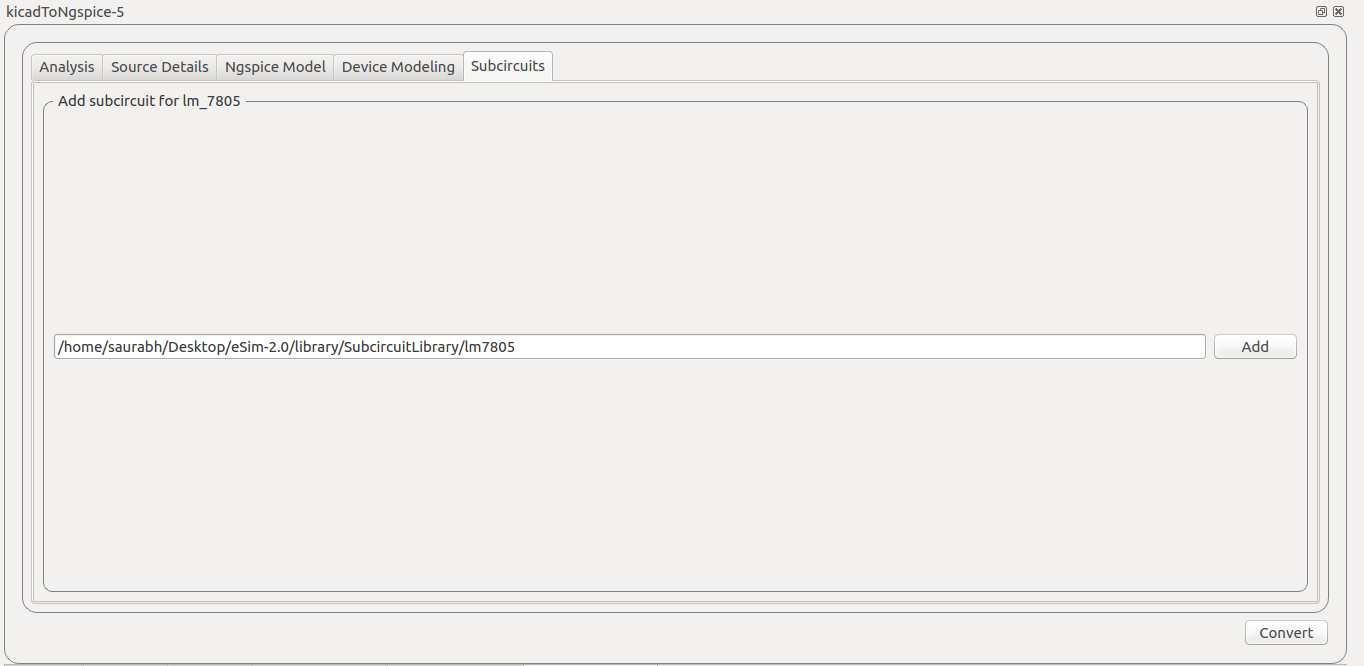
\includegraphics[width=\lgfig]{7805.png}
\caption{Assigning appropriate subcircuit file }
\label{7805}
\end{figure}
\\
\begin{comment}
The field in this tab are added for each such component in the circuit and the corresponding subcirucit is added. . as shown in \figref{bridgerectifier} for component Half_Adder the file is added as in \figref{devicemodel}.  
-------Just need to change the images------------
\begin{figure}[h]
\centering
\subfloat[Schematic]{
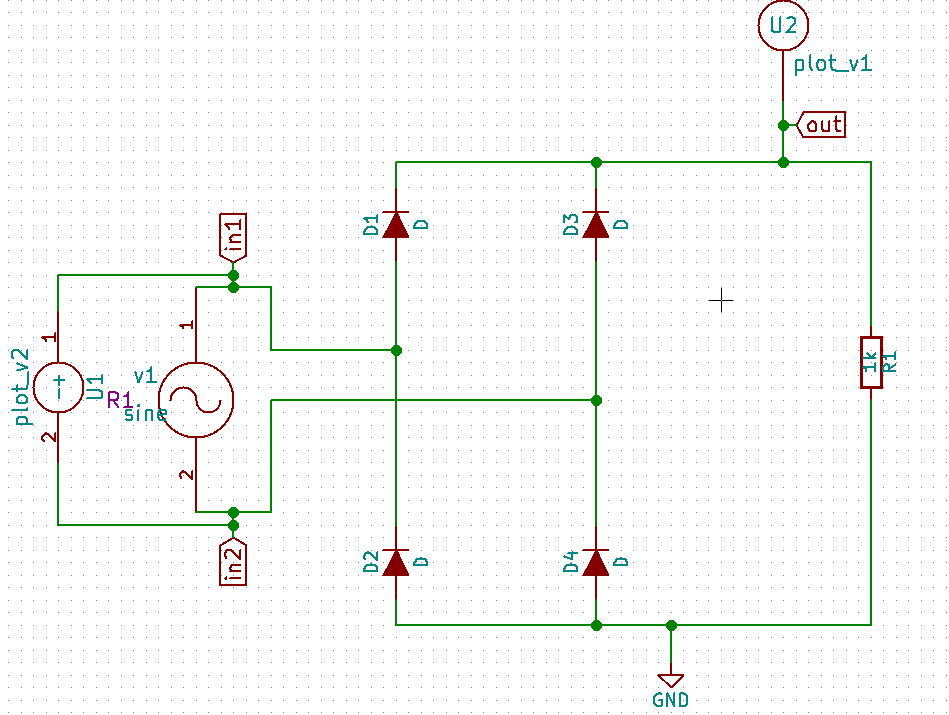
\includegraphics[width=\smfig]{manual_images/bridgerectifier.png}
\label{bridgerectifier}} \hfill
\subfloat[Adding device model]{
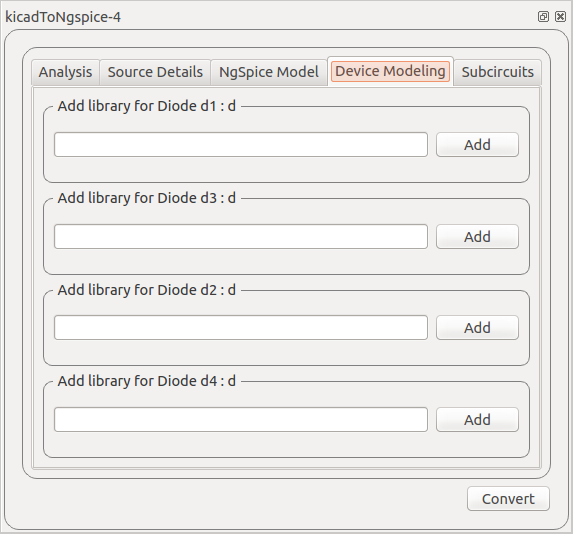
\includegraphics[width=\smfig]{manual_images/devicemodel.png}
\label{devicemodel}} \hfill
\caption{Bridge Rectifier}
\end{figure}
\end{comment}


After Filling up the values in all the above mentioned fields the convert button is pressed. The Ngspice netlist, {\tt .cir.out} file is generated. A message box pops up, as shown in \figref{success}. Click on {\tt OK}.

\begin{figure}
\centering
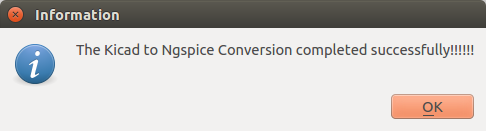
\includegraphics[width=\lgfig]{manual_images/success.png}
\caption{Message after successful Ngspice netlist generation}
\label{success}
\end{figure}

\section{Simulating the schematic}
\subsection{Simulation}
Once the Kicad to Ngspice conversion is successfully completed, press the \textit{Simulation} button on the leftside toolbar on eSim interface. This will display the Python plot window along with the node names. Select the required nodes and click on {\tt Plot}. The simulations are displayed. In the present example of the RC circuit, the plot will be displayed as shown in \figref{rc-python}.  By changing the values of capacitor and resistor, the output can be varied.We can also use the option {\tt Function} from the right side of the python plot window to plot combination of waveforms for example {\tt plot V1+V2}.

\begin{figure}
\centering
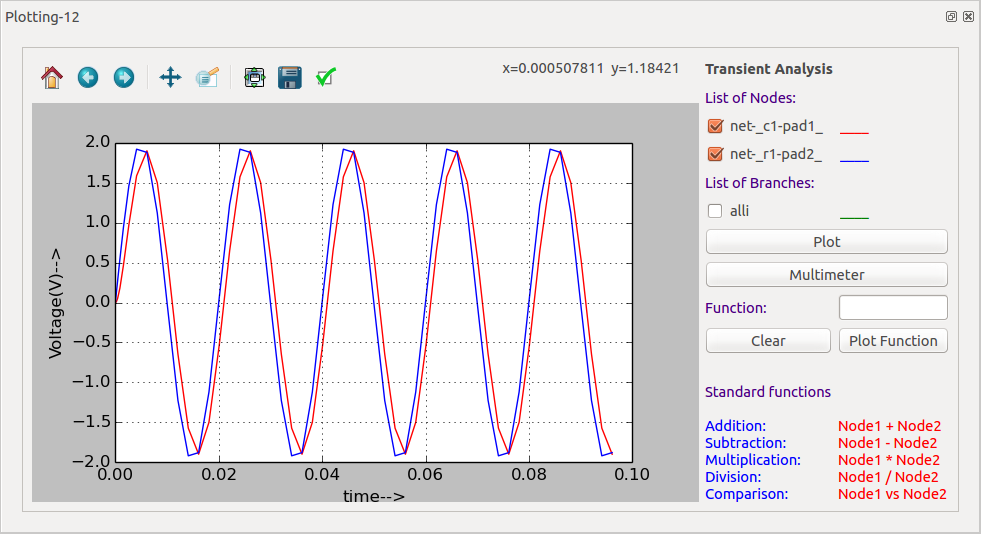
\includegraphics[width=\lgfig]{manual_images/rc-python.png}
\caption{Pythonplot for RC circuit}
\label{rc-python}
\end{figure}

Pressing the \textit{Simulation} button also opens up the Ngspice terminal and plot windows. The Ngspice plots for all the nodes (where we have used the plot components in the schematic) will be displayed. In the current example, we have used two plot components and the Ngspice simulations for these two nodes are displayed as in \figref{rc-voltage}.

\begin{figure}
\centering
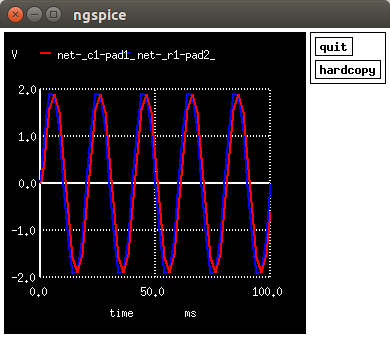
\includegraphics[width=\lgfig]{manual_images/rc-voltage.png}
\caption{Ngspice voltage simulation for RC circuit}
\label{rc-voltage}
\end{figure}

If the \textit{Plot components} are not used in the schematic, the simulations are not displayed automatically. To see the Ngspice simulations, type the following commands in the Ngspice terminal window.
\begin{itemize}
\item \textbf{plot allv} - Plots all the voltage waveforms.
\item \textbf{plot v(node-name)} - Plot a waveform of the node-name voltage source e.g. \textbf{plot v(out)} will plot the voltage at node \textbf{out} 
\item \textbf{plot v(node-one) v(node-two)} - Plots waveforms of voltages at node-one and node-two on a single graph. Multiple nodes can be observed in a single graph, though scaling has to be kept in mind. 
\item \textbf{plot alli} - Plots all the current waveforms.

You can refer the ngspice commands from {\tt https://esim.fossee.in/ngspicecmd}
\end{itemize}

\subsection{Multimeter}
Multimeter is another feature that is available in eSim. Using this facility the user can view the voltage and current values in various nodes and branches respectively. To use the multimeter select the required nodes from the plot window and press {\tt Multimeter} button, shown in \figref{multimeter}. Windows equal to the number of selected nodes will open. Now open the schematic window and place these pop up windows near the appropriate nodes on the schematic to get the voltage of each node. Similarly current through each branches in the schematic can also be found using the multimeter facility.

\begin{figure}
\centering
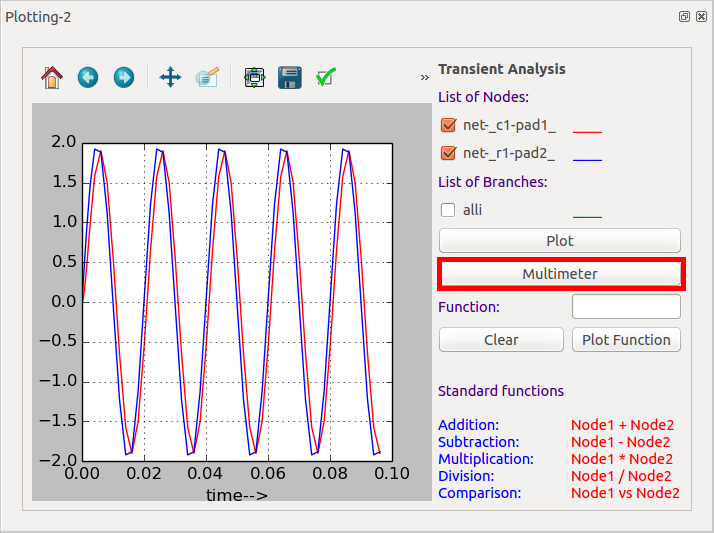
\includegraphics[width=\lgfig]{manual_images/multimeter.png}
\caption{Multimeter feature in eSim}
\label{multimeter}
\end{figure}


